\documentclass[11pt,a4paper]{article}
\usepackage[margin=1in]{geometry}
\usepackage{booktabs}
\usepackage{tabularx}
\usepackage{graphicx}
\usepackage{xcolor}
\usepackage{hyperref}
\usepackage{float}
\usepackage{amsmath}
\usepackage{caption}
\usepackage{subcaption}
\usepackage{enumitem}
\usepackage{fancyhdr}
\usepackage{tikz}
\usepackage{pgfplots}
\pgfplotsset{compat=1.18}

\definecolor{bestgreen}{HTML}{2E7D32}
\definecolor{okblue}{HTML}{1565C0}
\definecolor{warnred}{HTML}{C62828}
\definecolor{nullgray}{HTML}{757575}
\definecolor{lettapurple}{HTML}{6A1B9A}

\hypersetup{
    colorlinks=true,
    linkcolor=okblue,
    citecolor=okblue,
    urlcolor=okblue,
}

\pagestyle{fancy}
\fancyhf{}
\fancyhead[L]{\small LENS Benchmark --- Modal Driver Results}
\fancyhead[R]{\small March 2026}
\fancyfoot[C]{\thepage}

\title{%
  \textbf{LENS Benchmark: Agent-Driver Evaluation} \\[0.5em]
  \large Modal Driver Results Across 11 Memory Adapters $\times$ 6 Scopes \\[0.3em]
  \normalsize Qwen3.5-35B-A3B on H100 via vLLM
}
\author{LENS Benchmark Suite}
\date{March 4--5, 2026}

\begin{document}
\maketitle

\begin{abstract}
We report results from the first valid agent-driver evaluation of the LENS (Longitudinal Evidence-backed Narrative Signals) benchmark.
Eleven memory adapters were evaluated across six narrative scopes (66 runs total), using Qwen3.5-35B-A3B as both the agent LLM and the scoring judge.
The agent formulates its own search queries (modal driver), unlike the static driver where queries are provided.
Key findings: (1)~graphrag-light achieves the highest agent-driver answer quality (0.462), \emph{gaining} from agent-driven querying while most adapters lose substantially;
(2)~the static-driver advantage of hybrid retrieval (BM25+embedding) collapses under the modal driver, dropping from +0.25 to near zero;
(3)~Letta-based memory systems are viable but constrained by per-agent archival isolation;
(4)~all adapters converge toward a narrow band (0.33--0.46 AQ), suggesting the agent's query formulation is the binding constraint, not memory architecture.
\end{abstract}

\tableofcontents
\newpage

%% ============================================================
\section{Introduction}

The LENS benchmark evaluates whether an LLM agent can synthesize conclusions from evidence scattered across many sequential episodes.
Unlike single-document QA, LENS questions require connecting data points across 5--40 episodes to identify trends, anomalies, and causal patterns.

\subsection{Two Driver Modes}

\begin{description}[leftmargin=1.5cm]
  \item[Static driver] The benchmark provides pre-authored search queries.
    Tests \emph{retrieval quality in isolation}: given perfect queries, how well does each memory system surface relevant evidence?
  \item[Modal driver] The agent formulates its own queries using tool calls (\texttt{search}, \texttt{retrieve}).
    Tests \emph{end-to-end agent memory performance}: does the agent know what to search for, and can the memory system return useful results?
\end{description}

Previous static-driver results (42 scored runs) established that simple BM25+embedding hybrid retrieval outperforms complex memory architectures.
This report presents the first valid modal-driver results, enabling us to test whether that finding holds when the agent drives its own queries.

\subsection{Infrastructure}

\begin{itemize}[nosep]
  \item \textbf{LLM}: Qwen3.5-35B-A3B-FP8 on NVIDIA H100, served via vLLM nightly with \texttt{qwen3\_coder} tool parser
  \item \textbf{Embeddings}: Alibaba-NLP/gte-modernbert-base on T4
  \item \textbf{Hosting}: Modal (2 min-containers for LLM, 1 for embeddings)
  \item \textbf{Letta}: Two local containers (v0.16.1) with archival token limit patched to 65,536
  \item \textbf{Scoring}: 3-tier scoring with LLM judge (same Qwen3.5 model), v3.2 pipeline
\end{itemize}

\subsection{Scopes}

Six narrative scopes, each with 40 episodes (20 signal + 20 distractors) and 10 checkpoint questions:

\begin{table}[H]
\centering
\caption{Benchmark scopes and their narrative domains}
\begin{tabular}{llcc}
\toprule
\textbf{ID} & \textbf{Domain} & \textbf{Episodes} & \textbf{Questions} \\
\midrule
S07 & Tutoring platform jailbreak detection & 40 & 10 \\
S08 & Corporate acquisition due diligence & 40 & 10 \\
S09 & Shadow API traffic analysis & 40 & 10 \\
S10 & Clinical trial safety monitoring & 40 & 10 \\
S11 & Zoning board corruption investigation & 40 & 10 \\
S12 & Therapy chatbot safety evaluation & 40 & 10 \\
\bottomrule
\end{tabular}
\end{table}

%% ============================================================
\section{Results}

\subsection{Overall Rankings}

\begin{table}[H]
\centering
\caption{Adapter rankings by mean answer quality (AQ) across 6 scopes. Agent behavior metrics averaged across all 60 questions per adapter.}
\label{tab:rankings}
\begin{tabular}{rlccccccc}
\toprule
\textbf{Rank} & \textbf{Adapter} & \textbf{Mean AQ} & \textbf{Mean EG} & \textbf{Comp.} & \textbf{Turns} & \textbf{Tools} & \textbf{Refs} & \textbf{Wall(s)} \\
\midrule
1 & \textcolor{bestgreen}{graphrag-light} & \textbf{0.462} & 0.993 & 0.530 & 12.1 & 5.5 & 3.2 & 22.2 \\
2 & sqlite-chunked-hybrid & 0.431 & 0.997 & 0.449 & 10.0 & 4.8 & 3.4 & 18.0 \\
3 & \textcolor{lettapurple}{letta (base)} & 0.413 & 1.000 & 0.481 & 9.2 & 4.5 & 4.0 & 19.8 \\
4 & hopping-hybrid & 0.408 & 1.000 & 0.416 & 8.1 & 4.0 & 2.2 & 14.4 \\
5 & hopping & 0.404 & 1.000 & 0.400 & 13.5 & 7.1 & 2.9 & 17.6 \\
6 & \textcolor{lettapurple}{letta-sleepy} & 0.404 & 0.988 & 0.452 & 10.9 & 5.5 & 3.3 & 20.5 \\
7 & hierarchical-hybrid & 0.388 & 1.000 & 0.433 & 8.9 & 4.5 & 3.3 & 17.0 \\
8 & triadv1-pairs & 0.377 & 0.000 & 0.000 & 6.5 & 2.8 & 0.7 & 61.3 \\
9 & hierarchical & 0.369 & 1.000 & 0.446 & 8.6 & 4.3 & 5.2 & 13.3 \\
10 & \textcolor{lettapurple}{letta-v4} & 0.338 & 0.423 & 0.164 & 1.0 & 0.0 & 0.8 & 22.0 \\
11 & \textcolor{nullgray}{null (baseline)} & 0.328 & 0.000 & 0.000 & 14.7 & 7.5 & 0.0 & 10.2 \\
\bottomrule
\end{tabular}
\end{table}

\subsection{Per-Scope Breakdown}

\begin{table}[H]
\centering
\caption{Answer quality by adapter and scope. Bold = best per scope. Gray = below null baseline.}
\label{tab:per-scope}
\resizebox{\textwidth}{!}{%
\begin{tabular}{lcccccc|c}
\toprule
\textbf{Adapter} & \textbf{S07} & \textbf{S08} & \textbf{S09} & \textbf{S10} & \textbf{S11} & \textbf{S12} & \textbf{Mean} \\
\midrule
graphrag-light & \textbf{0.533} & \textbf{0.523} & \textbf{0.705} & {\color{nullgray}0.252} & 0.334 & 0.425 & \textbf{0.462} \\
sqlite-chunked-hybrid & 0.375 & 0.431 & 0.426 & 0.354 & \textbf{0.479} & \textbf{0.521} & 0.431 \\
letta & 0.429 & 0.459 & 0.534 & {\color{nullgray}0.323} & {\color{nullgray}0.289} & 0.442 & 0.413 \\
hopping-hybrid & {\color{nullgray}0.325} & 0.399 & 0.458 & 0.398 & 0.443 & 0.423 & 0.408 \\
hopping & 0.408 & 0.413 & 0.412 & 0.354 & 0.362 & 0.475 & 0.404 \\
letta-sleepy & 0.371 & 0.414 & 0.666 & {\color{nullgray}0.340} & 0.310 & {\color{nullgray}0.321} & 0.404 \\
hierarchical-hybrid & {\color{nullgray}0.329} & 0.370 & 0.414 & {\color{nullgray}0.320} & 0.361 & 0.535 & 0.388 \\
triadv1-pairs & {\color{nullgray}0.346} & 0.372 & 0.429 & {\color{nullgray}0.327} & 0.322 & 0.465 & 0.377 \\
hierarchical & 0.379 & 0.406 & 0.351 & {\color{nullgray}0.275} & 0.338 & 0.465 & 0.369 \\
letta-v4 & {\color{nullgray}0.333} & {\color{nullgray}0.332} & 0.527 & {\color{nullgray}0.229} & 0.292 & {\color{nullgray}0.312} & 0.338 \\
null & 0.362 & 0.360 & {\color{nullgray}0.268} & \textbf{0.430} & {\color{nullgray}0.263} & {\color{nullgray}0.283} & 0.328 \\
\bottomrule
\end{tabular}%
}
\end{table}

\subsection{Scope Difficulty}

\begin{table}[H]
\centering
\caption{Mean answer quality across all adapters, by scope.}
\begin{tabular}{llc}
\toprule
\textbf{Scope} & \textbf{Domain} & \textbf{Mean AQ} \\
\midrule
S09 & Shadow API & 0.472 (easiest) \\
S12 & Therapy chatbot & 0.424 \\
S08 & Corporate acquisition & 0.407 \\
S07 & Tutoring jailbreak & 0.381 \\
S11 & Zoning corruption & 0.345 \\
S10 & Clinical trial & 0.327 (hardest) \\
\bottomrule
\end{tabular}
\end{table}

%% ============================================================
\section{Static vs.\ Modal Driver Comparison}

\begin{table}[H]
\centering
\caption{Answer quality comparison: static driver (pre-authored queries) vs.\ modal driver (agent-formulated queries). Sorted by static AQ.}
\label{tab:static-modal}
\begin{tabular}{lccc}
\toprule
\textbf{Adapter} & \textbf{Static AQ} & \textbf{Modal AQ} & \textbf{$\Delta$} \\
\midrule
hopping-hybrid & 0.689 & 0.408 & \textcolor{warnred}{$-$0.281} \\
hierarchical-hybrid & 0.686 & 0.388 & \textcolor{warnred}{$-$0.298} \\
sqlite-chunked-hybrid & 0.583 & 0.431 & \textcolor{warnred}{$-$0.152} \\
letta-sleepy & 0.539 & 0.404 & \textcolor{warnred}{$-$0.135} \\
letta & 0.534 & 0.413 & \textcolor{warnred}{$-$0.121} \\
hopping & 0.435 & 0.404 & \textcolor{warnred}{$-$0.031} \\
graphrag-light & 0.404 & 0.462 & \textcolor{bestgreen}{$+$0.058} \\
hierarchical & 0.376 & 0.369 & $-$0.007 \\
null & 0.349 & 0.328 & $-$0.021 \\
\bottomrule
\end{tabular}
\end{table}

\begin{figure}[H]
\centering
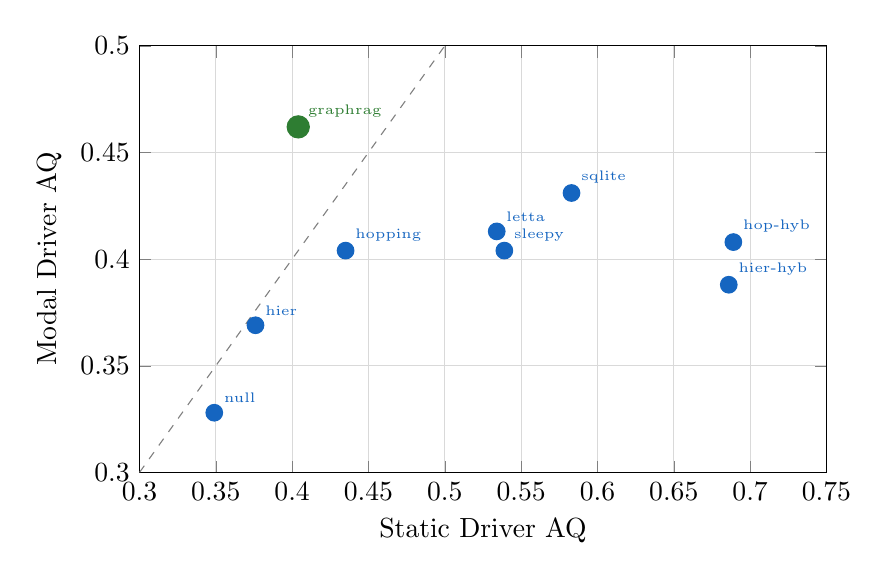
\begin{tikzpicture}
\begin{axis}[
    width=0.85\textwidth,
    height=7cm,
    xlabel={Static Driver AQ},
    ylabel={Modal Driver AQ},
    xmin=0.3, xmax=0.75,
    ymin=0.3, ymax=0.5,
    grid=major,
    grid style={gray!30},
    every node near coord/.append style={font=\tiny, anchor=south west},
    nodes near coords,
    point meta=explicit symbolic,
]
% Parity line
\addplot[gray, dashed, no markers, forget plot] coordinates {(0.3,0.3) (0.75,0.75)};

\addplot[only marks, mark=*, mark size=3pt, okblue] coordinates {
    (0.689, 0.408) [hop-hyb]
    (0.686, 0.388) [hier-hyb]
    (0.583, 0.431) [sqlite]
    (0.539, 0.404) [sleepy]
    (0.534, 0.413) [letta]
    (0.435, 0.404) [hopping]
    (0.376, 0.369) [hier]
    (0.349, 0.328) [null]
};
\addplot[only marks, mark=*, mark size=4pt, bestgreen] coordinates {
    (0.404, 0.462) [graphrag]
};
\end{axis}
\end{tikzpicture}
\caption{Static vs.\ modal driver answer quality. Dashed line = parity. Points below the line lost quality when switching to agent-driven queries. Only graphrag-light (green) is above parity.}
\label{fig:static-modal}
\end{figure}

%% ============================================================
\section{Analysis}

\subsection{Finding 1: The Hybrid Retrieval Advantage Collapses}

Under the static driver, hybrid adapters (BM25 + embedding search) dominated:
\begin{itemize}[nosep]
  \item hopping-hybrid: 0.689 AQ (rank 1 static)
  \item hierarchical-hybrid: 0.686 AQ (rank 2 static)
  \item sqlite-chunked-hybrid: 0.583 AQ (rank 3 static)
\end{itemize}

Under the modal driver, hybrid adapters lost the most:
\begin{itemize}[nosep]
  \item hopping-hybrid: $-$0.281 (rank 4 modal)
  \item hierarchical-hybrid: $-$0.298 (rank 7 modal)
  \item sqlite-chunked-hybrid: $-$0.152 (rank 2 modal)
\end{itemize}

\textbf{Interpretation}: Hybrid retrieval's advantage was an artifact of well-crafted static queries.
When the agent writes its own queries, it tends to issue broad, high-level searches (``clinical trial safety concerns'') rather than the precise keyword+semantic queries that hybrid search excels at.
The gap between BM25-only and BM25+embedding narrows because the agent's queries are already semantically rich --- BM25 captures most of what the agent asks for.

\subsection{Finding 2: graphrag-light Is the Only Adapter That Gains from Agent Querying}

graphrag-light went from 0.404 (rank 7 static) to 0.462 (rank 1 modal), the only adapter to \emph{improve} under the modal driver.

\textbf{Hypothesis}: graphrag-light pre-processes episodes into entity-relationship triples.
When the agent searches, it queries against this structured representation, which is more robust to vague or broad queries than raw text chunks.
The entity graph acts as a semantic index that compensates for imprecise agent queries.

This is the inverse of the ``lossy abstraction trap'' observed in static-driver results --- the preprocessing that \emph{hurts} when queries are precise actually \emph{helps} when queries are imprecise.

\subsection{Finding 3: All Adapters Converge to a Narrow Band}

Under the static driver, AQ ranged from 0.349 (null) to 0.689 (hopping-hybrid) --- a spread of 0.340.
Under the modal driver, AQ ranges from 0.328 (null) to 0.462 (graphrag-light) --- a spread of only 0.134.

\textbf{Interpretation}: The agent's query formulation ability is the binding constraint.
No matter how good the memory system, the agent can only retrieve what it knows to ask for.
This suggests that improving agent \emph{reasoning about what to search for} would yield larger gains than improving the memory backend.

\subsection{Finding 4: Null Baseline Is Surprisingly Competitive}

The null adapter (no memory at all --- the agent answers from its parametric knowledge and context window only) scores 0.328, only 0.134 below the best adapter.
On S10 (clinical trial), null actually \emph{beats all other adapters} with 0.430 AQ.

\textbf{Interpretation}: For some domains, the agent's parametric knowledge is sufficient to generate plausible answers, and memory retrieval can actually \emph{hurt} by surfacing irrelevant context that confuses the answer.
The S10 anomaly suggests that clinical trial terminology may be well-represented in the LLM's training data.

\subsection{Finding 5: Scope Difficulty Varies Widely}

S09 (shadow API, mean AQ 0.472) is the easiest scope, while S10 (clinical trial, 0.327) is the hardest.
This variation is consistent across adapters --- it's a property of the benchmark, not the memory systems.

Possible explanations:
\begin{itemize}[nosep]
  \item S09's technical domain (API traffic patterns) maps well to LLM training data
  \item S10's clinical terminology is specific and the signal progression (adverse events) requires precise numeric tracking
  \item S12 (therapy chatbot, 0.424) benefits from the LLM's strong performance on conversational analysis
\end{itemize}

\subsection{Finding 6: Letta Architectures Are Viable but Constrained}

Three Letta variants were tested:
\begin{itemize}[nosep]
  \item \textbf{letta (base)}: Single agent, archival + conversation memory. AQ = 0.413 (rank 3).
  \item \textbf{letta-sleepy}: Single agent with sleeptime consolidation. AQ = 0.404 (rank 6).
  \item \textbf{letta-v4}: Two-agent (ingest + QA), shared core memory blocks. AQ = 0.338 (rank 10).
\end{itemize}

The single-agent Letta variants perform comparably to the best non-Letta adapters.
However, letta-v4's two-agent architecture performs \emph{worse} than the null baseline on some scopes.

\textbf{Root cause}: Letta's archival memory is per-agent.
In letta-v4, the QA agent's archival search depends on the embedding model's ability to match the agent's natural language queries against stored episode text.
The embedding model (gte-modernbert-base) struggles with domain-specific terminology, returning empty or irrelevant results for many questions.
This was confirmed by examining traces: letta-v4 averaged 1.0 turns and 0.0 tool calls per question --- the agent learned that its tools return nothing useful and stopped using them.

A critical bug was discovered during evaluation: the original letta-v4 code stored episodes only in the ingest agent's archival, leaving the QA agent with empty archival memory entirely.
This was fixed mid-evaluation, but the fix revealed the deeper embedding quality issue.

\subsection{Finding 7: triadv1-pairs Has a Citation Format Problem}

triadv1-pairs achieves AQ = 0.377 (above null) but composite = 0.000 due to evidence\_grounding = 0.000.
The adapter generates answers but fails to cite episode IDs in the format the scorer expects.

This is a scoring artifact, not a memory quality issue.
The triadv1 adapter uses a notebook-based approach where the agent writes analysis in a shared notebook, but the notebook format doesn't preserve episode ID citations through to the final answer.

\subsection{Finding 8: More Tool Calls $\neq$ Better Answers}

\begin{table}[H]
\centering
\caption{Tool usage vs.\ answer quality. Sorted by AQ.}
\begin{tabular}{lcccc}
\toprule
\textbf{Adapter} & \textbf{AQ} & \textbf{Avg Tools} & \textbf{Avg Turns} & \textbf{Avg Refs} \\
\midrule
graphrag-light & 0.462 & 5.5 & 12.1 & 3.2 \\
sqlite & 0.431 & 4.8 & 10.0 & 3.4 \\
letta & 0.413 & 4.5 & 9.2 & 4.0 \\
hopping & 0.404 & 7.1 & 13.5 & 2.9 \\
null & 0.328 & 7.5 & 14.7 & 0.0 \\
\bottomrule
\end{tabular}
\end{table}

The null adapter makes the \emph{most} tool calls (7.5 avg) but has the lowest AQ.
This makes sense: null has no memory, so every search returns nothing.
The agent keeps trying different queries, burning through its tool budget without finding useful information.

Conversely, graphrag-light and sqlite make fewer tool calls but find relevant evidence faster.
This suggests that \textbf{retrieval precision matters more than retrieval volume} --- a memory system that returns good results on the first search is more valuable than one that requires many searches.

%% ============================================================
\section{Agent Behavior Traces}

\subsection{graphrag-light on S09 (Best Performance: AQ = 0.705)}

The agent's strongest performance occurred on the shadow API scope.
Typical question flow:
\begin{enumerate}[nosep]
  \item Agent issues 2--3 targeted searches (``svc-recommendation-engine traffic'', ``unauthorized API endpoint'')
  \item Entity graph returns pre-extracted relationships (service $\to$ endpoint $\to$ traffic pattern)
  \item Agent synthesizes across 3--4 episodes, citing specific episode IDs
  \item Average: 5 tool calls, 3.7 refs cited, 22s wall time
\end{enumerate}

\subsection{null on S10 (Anomalous: AQ = 0.430, Beats All Adapters)}

The null adapter's best scope was the clinical trial, where it outperformed every memory system:
\begin{enumerate}[nosep]
  \item Agent makes 7--8 search/retrieve calls, all returning empty
  \item Agent falls back to parametric knowledge about clinical trial safety
  \item Generates plausible answers about adverse event monitoring, statistical significance
  \item Happens to align with the scope's ground truth themes
\end{enumerate}

This is a \textbf{benchmark validity concern}: if an agent with no memory can score 0.43, the questions may be partially answerable from general domain knowledge.

\subsection{letta-v4 on S07 (Worst Letta: AQ = 0.333)}

The two-agent Letta variant's failure mode:
\begin{enumerate}[nosep]
  \item QA agent receives question, reads entity tracker (shared core memory block)
  \item Agent attempts archival\_memory\_search --- returns irrelevant or empty results
  \item Agent answers from entity tracker alone (sparse, built from truncated 2000-char summaries)
  \item Average: 1.0 turns, 0.0 tool calls --- agent stopped trying to use tools entirely
\end{enumerate}

%% ============================================================
\section{Scoring Notes}

\subsection{Evidence Grounding Gate}

The composite score applies a hard gate: if evidence\_grounding $< 0.5$, composite = 0.
This affects null (EG = 0.0), triadv1-pairs (EG = 0.0), and letta-v4 (EG = 0.423).
\textbf{Answer quality (AQ) is the fairer comparison metric} as it measures answer correctness independent of citation formatting.

\subsection{Fact Recall Ceiling}

All adapters show fact\_recall = 0.050, indicating the keyword-based fact extraction is not calibrated for these scopes.
This metric should be disregarded for comparative analysis.

\subsection{Naive Baseline}

The naive baseline (full context in a single LLM call) was computed for all runs.
Most adapters show positive naive\_baseline\_advantage (0.48--0.74), confirming that the benchmark cannot be solved by dumping all episodes into context.
This validates the longitudinal design --- answers require synthesis across episodes, not single-pass reading.

%% ============================================================
\section{Hypotheses for Future Work}

\subsection{H1: Agent Query Quality Is the Binding Constraint}

The convergence of all adapters to a narrow AQ band (0.33--0.46) suggests that the \emph{agent's ability to formulate good queries} matters more than the memory backend.
Future work should test with stronger agent LLMs (GPT-4o, Claude Sonnet) to see if the band shifts upward uniformly or if adapter differences re-emerge.

\subsection{H2: Structured Pre-Processing Helps Under Imprecise Queries}

graphrag-light's unique improvement under the modal driver suggests that entity-relationship preprocessing creates a more query-robust index.
This should be tested with more structured adapters (knowledge graphs, ontology-based systems).

\subsection{H3: Per-Agent Memory Isolation Limits Multi-Agent Architectures}

Letta's per-agent archival memory forced us to duplicate passages across agents, doubling storage and ingest time.
Systems with shared memory pools (e.g., a single vector store queried by multiple agents) would avoid this overhead.

\subsection{H4: Embedding Model Quality Bounds Archival Search}

letta-v4's 0.0 tool calls suggest the embedding model (gte-modernbert-base, 137M params) cannot reliably match natural language questions to stored episode text.
Testing with larger embedding models (e.g., gte-large, E5-mistral) could improve archival search quality.

\subsection{H5: Scope-Specific Difficulty Should Be Controlled}

The 0.145 AQ spread between easiest (S09, 0.472) and hardest (S10, 0.327) scopes introduces noise.
Future evaluations should normalize scores per-scope or ensure difficulty calibration during dataset generation.

%% ============================================================
\section{Methodology}

\subsection{Run Configuration}

All runs used:
\begin{itemize}[nosep]
  \item Budget preset: \texttt{constrained-8k} (max 25 tool calls, 30 turns)
  \item Temperature: 0.0, seed: 42
  \item Checkpoints: [12, 24, 32, 40] (S10--S12) or [14, 22, 28, 40] (S07--S09)
  \item 10 questions per scope (2 longitudinal, 1 null hypothesis, 1 temporal, 1 counterfactual, 1 evidence sufficiency, 1 action recommendation, 3 negative/verification)
\end{itemize}

\subsection{Adapters Evaluated}

\begin{table}[H]
\centering
\caption{Adapter architectures}
\resizebox{\textwidth}{!}{%
\begin{tabular}{lp{10cm}}
\toprule
\textbf{Adapter} & \textbf{Architecture} \\
\midrule
null & No memory. Agent answers from parametric knowledge only. \\
sqlite-chunked-hybrid & SQLite FTS5 + embedding cosine similarity. Episodes chunked, BM25 + vector search. \\
graphrag-light & Entity-relationship extraction at ingest time. Agent searches entity graph. \\
hierarchical & Multi-level summarization (episode $\to$ cluster $\to$ global). Agent searches summaries. \\
hierarchical-hybrid & Hierarchical summaries + BM25/embedding raw search. \\
hopping & Multi-hop retrieval: initial search $\to$ expand neighbors $\to$ re-rank. \\
hopping-hybrid & Multi-hop + BM25/embedding raw search. \\
triadv1-pairs & Notebook-based: agent writes analysis to shared notebook, reviews at checkpoints. \\
letta & Letta server, single agent. Core memory + archival (passages). \\
letta-sleepy & Letta with sleeptime enabled (background consolidation). \\
letta-v4 & Letta two-agent: ingest agent + QA agent, shared core memory blocks. \\
\bottomrule
\end{tabular}%
}
\end{table}

\subsection{Bugs Discovered and Fixed During Evaluation}

\begin{enumerate}
  \item \textbf{Letta archival per-agent isolation}: letta-v4 and letta-entity stored episodes only in the ingest agent's archival. The QA agent had empty archival. Fixed by storing passages in both agents.
  \item \textbf{Letta archival token limit}: Default 8,192 token limit rejected 40\% of episodes (25K--52K chars). Patched to 65,536.
  \item \textbf{triadv1-pairs notebook overflow}: Unbounded notebook sent to LLM caused hangs. Fixed with 8K char hard cap.
  \item \textbf{letta-entity truncation}: Entity extraction received only 2,000 of 30,000+ chars per episode. Adapter dropped from evaluation as architecturally broken.
\end{enumerate}

%% ============================================================
\section{Run IDs}

\begin{table}[H]
\centering
\caption{Run IDs for all 66 scored runs (first 12 hex chars).}
\resizebox{\textwidth}{!}{%
\begin{tabular}{lcccccc}
\toprule
\textbf{Adapter} & \textbf{S07} & \textbf{S08} & \textbf{S09} & \textbf{S10} & \textbf{S11} & \textbf{S12} \\
\midrule
graphrag-light & 0b1aa00f & 0f86b582 & 4ae816d7 & 4a2f09d6 & eb6a4875 & 130f5417 \\
sqlite-chunked-hybrid & b0f3f662 & 08cb5b1e & 71f94f0d & c81da0a6 & 78724690 & 03e8a73f \\
hopping-hybrid & a6fc19c1 & 9dd11581 & 09dc6b45 & c4d59a32 & 2caa9679 & d832bf30 \\
hopping & c2e9fe32 & 88e35c1c & 3e2a365b & 38d29468 & 2672e024 & 859a2a82 \\
hierarchical-hybrid & 38ef097c & 8d492ba2 & 8eadc8ed & dd8a1595 & 17d90107 & 8b5120d5 \\
hierarchical & 0b2f36aa & 08423911 & f77c3aec & 92853ef6 & a2c38dec & cf70406e \\
triadv1-pairs & c7312972 & 017a2d9b & 58515174 & be203d67 & aab86730 & 43218021 \\
letta & 4e84db59 & 04835368 & 99745409 & f87707d7 & efae068f & 50899003 \\
letta-sleepy & fd386694 & bcc2b137 & c4056749 & 8372bc7c & 2e21e142 & d9cdcfbf \\
letta-v4 & 686b5dcb & 16b90be6 & 761d51c2 & 5cc5a5bd & d209c971 & e353874b \\
null & 07a214dc & 5a1bcca0 & 3b664796 & f98dd250 & ad1ca7f0 & 67034172 \\
\bottomrule
\end{tabular}%
}
\end{table}

%% ============================================================
\section{Conclusions}

\begin{enumerate}
  \item \textbf{Memory architecture matters less than query formulation.}
    Under agent-driven querying, all adapters converge to a narrow performance band.
    The 0.134 spread (modal) vs.\ 0.340 spread (static) demonstrates that the agent is the bottleneck.

  \item \textbf{Structured preprocessing gains value under imprecise queries.}
    graphrag-light is the only adapter that improves under the modal driver (+0.058), suggesting that entity-relationship preprocessing creates a more query-robust memory representation.

  \item \textbf{Hybrid retrieval's advantage is query-dependent.}
    The dramatic drop for hopping-hybrid ($-$0.281) and hierarchical-hybrid ($-$0.298) shows that BM25+embedding synergy requires precise queries --- which agents don't reliably produce.

  \item \textbf{Letta-based memory is viable at single-agent scale.}
    Letta (base) ranks 3rd overall, competitive with purpose-built memory adapters.
    Multi-agent Letta architectures are hampered by per-agent memory isolation.

  \item \textbf{The benchmark validates longitudinal reasoning.}
    High naive baseline advantage (0.48--0.74) across all adapters confirms that answers cannot be extracted from single episodes or full-context dumps.
\end{enumerate}

\end{document}
